\Titelbanner{10}{Integralrechnung}

\textbf{Aufgabe 1: } \emph{Stammfunktionen}\\[0.2cm]
Bestimmen Sie jeweils die Stammfunktion $F(x)$ der folgenden Funktionen.
\begin{align*}
&\text{(a)}\quad f(x)=\sin(2x+5)					&& \text{(b)}\quad f(x)=\frac{k}{kx+1}\\[1ex]
&\text{(c)}\quad f(x)=\frac{\cos(x)}{\sin(x)}		&& \text{(d)}\quad f(x)=\frac{a\cos(x)+b\sin(x)}{c\sin(x)}\\[1ex]
&\text{(e)}\quad f(x)=\frac{x^2+1}{x^2-1}			&& \text{(f)}\quad f(x)=\frac{kx}{\sqrt{x^2+y^2}^3}
\end{align*}
\emph{Hinweis:} Partialbruchzerlegung in (e).\\[1cm]
%
\textbf{Aufgabe 2: } \emph{Partielle Integration}\\[0.2cm]
Bestimmen Sie die folgenden Integrale unter Verwendung partieller Integration.
\begin{align*}
&\text{(a)}\quad \int\limits_0^\pi x\sin(x)\d x			&& \text{(b)}\quad \int\limits_0^1 x^3\e^{x}\d x\\[1ex]
&\text{(c)}\quad \int\limits_{r_0}^{2r_0} r\left(1+\ln\frac{r}{r_0}\right)\d r	&& \text{(d)}\quad \int\frac{\ln(x)}{x}\d x
\end{align*}\\[0.8cm]
%
\textbf{Aufgabe 3: } \emph{Substitutionen}\\[0.2cm]
Berechnen Sie die folgenden Integrale jeweils unter Verwendung der angegebenen Substitution.
\begin{align*}
&\text{(a)}\quad \int\limits_0^1 \sqrt{1-x^2}\d x\,,		&&\text{mit}\quad x=\sin\phi\\[1ex]
&\text{(b)}\quad \int\limits_0^1 \frac{\d x}{(1+x^2)\sqrt{\arctan(x)}}	\,,	&&\text{mit}\quad u=\arctan(x)
\end{align*}
%

\newpage\noindent
\textbf{Aufgabe 4: } \emph{Vollständige Induktion}\\[0.2cm]
Zeigen Sie mithilfe vollständiger Induktion, dass für die Fakultät $n! = n\cdot (n-1) \cdot \hdots \cdot 1$
\begin{align*}
        n! = \int\limits_{0}^{\infty} x^n \e^{-x} \dd{x},
\end{align*}
gilt. \emph{Hinweis}: Es gilt $0! = 1$.

\textbf{Aufgabe 5: } \emph{Flächenintegral}\\[0.2cm]
Leiten Sie die Formel für den Flächeninhalt eines Kreises vom Radius $R$ her.
\begin{center}
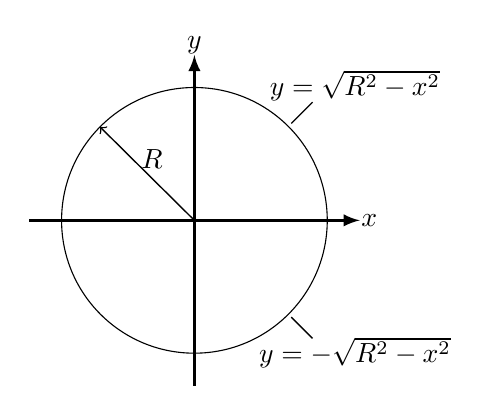
\begin{tikzpicture}[scale=0.6]
\draw[-{latex}, line width=1pt] (0,-3.5)--(0,3.5);
\draw[-{latex}, line width=1pt] (-3.5,0)--(3.5,0);
\draw (0,0) circle (80pt);
\node at (0,3.7) {$y$};
\node at (3.7,0) {$x$};
\draw[line width=0.5pt] (2.05,2.05)--(2.5,2.5);
\draw[line width=0.5pt] (2.05,-2.05)--(2.5,-2.5);
\node at (3.4,2.85) {$y=\sqrt{R^2-x^2}$};
\node at (3.4,-2.8) {$y=-\sqrt{R^2-x^2}$};
\draw[->,line width=0.5pt] (0,0)--(-2,1.98);
\node at (-0.9,1.3) {$R$};
\end{tikzpicture}
\end{center}
% \vspace{1cm}
%
\textbf{Aufgabe 6: } \emph{Volumenintegral}\\[0.2cm]
Berechnen Sie das Volumen des in der Abbildung gezeigten Körpers.\\
\begin{center}
\includegraphics[width=8cm]{koerper.pdf}
\end{center}
